\chapter{Power system}
\label{chap:power_system}
This chapter provides basic and fundamental components, laws and interconnections that lie behind any power system. All of them are used in derivation and composition of the systems' models and further optimization problems.
\section{Alternating Current Basics}

Power systems are built for transferring energy. This thesis considers electrical power systems which operates alternating current due to the victory of Nikola Tesla's alternating current over Thomas Edison's direct current way. Alternating current turned out to be more efficient in terms of losses in practice. This section explains basic physics behind alternating current using complex analysis elements.
\subsection{Phasors}

Phasor is a complex number that includes an amplitude, frequency and a phase shift. These complex numbers are used to describe alternating current, voltage and subsequent physical values that are used to compose a power system model. Specifically, for voltage $V(t)$ and current $I(t)$ the phasors are as follows:
\begin{equation}
    \begin{aligned}
        V(t) &= V_m e^{i(\omega t + \theta_v)}, \\
        I(t) &= I_m e^{i(\omega t + \theta_i)}.
    \end{aligned}
    \label{chapter_power_system:phasors}
\end{equation}
Here $V_m \in \mathbb{R}, I_m \in \mathbb{R}$ are voltage and current amplitude, $\omega$ is the grid frequency, $\theta_v, \theta_i$ are phase shifts \cite{machowski2020power}.
In Russia, Europe, Australia, Africa, Asia the grid frequency is $50$ Hz, while in American countries like Canada, USA, Mexico, Brazil the frequency is $60$ Hz. It is common that the are several harmonic signals in the grid with the same frequency, thus, it is convenient to denote a phasor in polar form, for voltage: $V(t)=V_m \angle\theta_v$, here temporal dependency is in the angle sign $\angle$. 
There are also rectangular $V(t) = V_m \cos(\omega t + \theta_v) + i V_m \sin(\omega t + \theta_v)$.
Such formulations are equivalent to each other and mean the same thing: a value of an alternating current or voltage at time step $t$. 

Since the current and voltage are interconnected it is convenient to use to the following notation:
\begin{equation}
    \begin{aligned}
        V(t) &= V_m e^{i\omega t}, \\
        I(t) &= I_m e^{i(\omega t - \phi)},
    \end{aligned}
    \label{chapter_power_system:phasors_shift}
\end{equation}
where $\phi = \theta_i - \theta_v$. Such notation is more convenient for further analysis and derivation of power system models.

\subsection{Electrical Power}

Electricity that is run through a circuit or a power system is typically expressed in terms of power in Watts (W) and describes the amount of energy (Joules, J) per time unit (second, s), thus, $[W] = \frac{[J]}{[s]}$. The amount of power consumer by a circuit element is calculated as a voltage drop: $S(t) = V(t) I(t)^*$, where $I(t)^*$ is a complex conjugate of voltage $I(t)$ \cite{el2008electric}. The power itself is a complex number, using \eqref{chapter_power_system:phasors_shift}:
\begin{equation}
        S(t) = V_m I_m e^{i\phi} = V_m I_m \cos \phi + i V_m I_m \sin \phi = P + i Q.        
    \label{chapter_power_system:apparent}
\end{equation}
The real part of the apparent power is called \emph{active power} (measured in Watts, W) and the imaginary part is called \emph{reactive power} (measured in Volt-Amperes, VAr). Active power is the part of total apparent power that can be used by consumers. On the other hand, the reactive power is the power that is exchanged between the electricity source and inductive or capacitive elements. 

\section{Power Grid}

In this section, fundamentals of alternating current are used to describe key components and interconnections of a power system using Kirchoff laws. The power flow analysis is essential for modeling a power system. It allows for calculating voltages, current, phases, power injection at buses in the whole system, opening a door for further generation optimization, market analysis and many other real-life related modeling problems \cite{machowski2020power}.


\subsection{Topological Model of a Power System}
A topology of a power grid is model by a graph. A graph is a set of edges and vertices, where edges can connect two edges \cite{zhuravlev1999discrete}. In power systems, vertices are buses that can contain a demand or a generator, edges represent power lines that are build for power transfer. Formally, speaking, let $\mathcal{B}$ be a set of buses and $\mathcal{L} \succ \mathcal{B} \times \mathcal{B}$ be a set of lines. Then the power system topologically is described as a graph $\mathcal{G} = (\mathcal{B}, \mathcal{L})$. The number of buses and lines as defined as cardinalities of the corresponding sets:
$$
\begin{aligned}
n_b &= |\mathcal{B}|, \\
n_l &= |\mathcal{L}|.
\end{aligned}
$$

\subsection{Bus Classification}

Buses in power system, that are nodes in the grid graph $\mathcal{G}$, are classified depending on their purpose in a power grid. They can either be a generator, load or slack bus. The ones that are not classified in these three, i.e., a transmission bus, are treated as a load with zero demand \cite{machowski2020power}. 
For a given power system state, a bus can be described using the complex voltage $V \in \mathbb{C}$ and the power injection $S \in \mathbb{C}$. The buses are classified based on the quantities of these complex numbers are known or must be defined using a power grid model. The classification is summarized in Table \ref{tab:bus_classif}
\begin{table}
\captionsetup{justification=centering}
\caption{Bus classification in a power grid}
\label{tab:bus_classif}
    \centering
        \begin{tabular} {p{3.5cm}p{4cm}p{2cm}}
        \toprule
        Bus type & Known variables & Unknown variables  \\
        \midrule
        PV-bus / generator & Active power $P$, voltage magnitude $V_m$ & Unknown variables  Phase angle $\phi$, reactive power $Q$ \\
        
        PQ / load & Active power $P$, reactive power $Q$ & Voltage magnitude $V_m$, phase angle $\phi$  \\

        Slack / swing & Voltage magnitude $V_m$, phase angle $\phi$  & Active power $P$, reactive power $Q$  \\
        
        \bottomrule
    \end{tabular}
\end{table}

\subsection{Power transmission lines}
Two buses that require a power transfer are connected with a power line. A transmission line characteristics can be quantities using the following four parameters \cite{machowski2020power}, noting that $\omega = 2 \pi f$ is the frequency in radians and $f$ is the frequency in Hz:
\begin{enumerate}
    \item Series resistance $r$ due to the wire conduct resistivity, per unit length
    \item Shunt conductance $g$ due to a leakage current between the ground and the phase, per unit length 
    \item Series reactance $x=\omega L$ due to a magnetic field surrounding the wires, per unit length, $L$ here is a series inductance, per unit length 
    \item Shunt susceptance $b^{sh}=\omega C$ due to an electric field between the wires, per unit length, $C$ here is the shut capacitance per unit length
\end{enumerate}

Thus, combining the series resistance and inductance one obtains a complex impedance $z = r + i x \in \mathcal{C}$. The shunt admittance is obtained via combination of conductance and capacitance $y = \frac{1}{z} = g + i b^{sh} \in \mathcal{C}$. Each of the components of these complex numbers represent a particular aspect of transmission line. The resistance $r$ represents the heating, in other words, Joule losses, the series impedance $L$ depends on the partial flux linkages between wire components and other nearby conductors. Next, the shunt conductance $g$ represents the corona loss and leakage currents on the insulators. Typically, $g$ is small for conductor lines and neglected. The shunt capacitance $C$ is due to the potential difference between the conductors, i.e., wires.
%page90

A power line is modeled using a $\pi$-model in power system steady-state analysis. The variables to analyse here are $V_R, I_R, V_S$ and $I_s$ -- voltages and currents at receiving and sending terminals (ends) of a power line. The $\pi$-model is illustrated in Figure \ref{fig:pi_model}. Here $Z_L$ is the total line impedance composed of resistance and reactance, in other words, $Z_L = (r + i x)l$, where $l$ is the line length, $Y_L$ is the shunt admittance where conductance component is neglected, i.e., $Y_L =i b^{sh} l$, where $l$ is the line length.

\begin{figure}
    \centering
    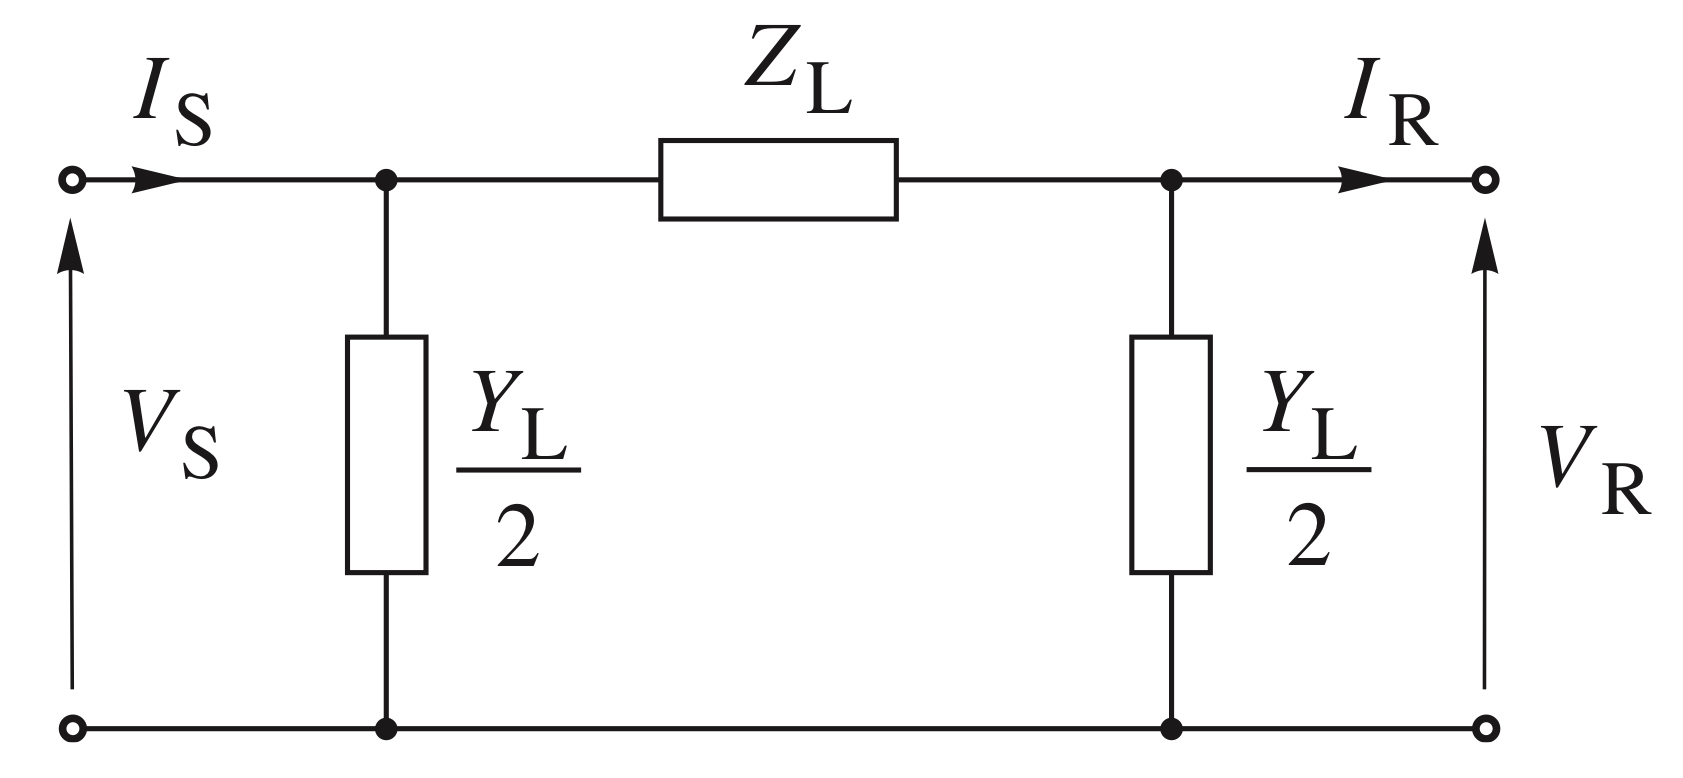
\includegraphics[width=0.9\textwidth]{Dissertation/images/pi_model.PNG}
    \caption{The $\pi$-equivalent of a power transmission line}
    \label{fig:pi_model}
\end{figure}

The receiving and sending physical quantities are linked via Kirchhoff law \cite{kirchhoff1847ueber}: 
$$
I_R = V_R \cdot Y_L/2 + (V_S - V_r) \cdot \frac{1}{Z_L}.
$$

\begin{comment}
The receiving voltages and current are linked between via long-line equation {\color{red} cite janusz, cite Power System Analysis: Grainger, John, Stevenson, William}:

\begin{equation}
    \begin{aligned}
        \begin{pmatrix}
            V_S  \\
            I_S 
        \end{pmatrix}
        =
        \begin{pmatrix}
            \cosh \gamma l      & Z_C \sinh \gamma l \\
            \sinh \gammal / Z_C & \cosh \gamma l
        \end{pmatrix}
        \begin{pmatrix}
            V_R  \\
            I_R 
        \end{pmatrix},
    \end{aligned}
    \label{eq:long-line}
\end{equation}
here $Z_C = \sqrt{z / y}$ is the characteristic, or surge, impedance of the power line and $\gamma = \sqrt{zy}$ is called the propagation constant.
\end{comment}

\subsection{Kirchhoff Current law and Admittance Matrix}

In the grid graph $\mathcal{G}$, a bus $b \in \mathbb{B}$ is connected to other buses $b' \in \textit{Adj}(b) = \{ b':~ \exists l = (b, b') ~\wedge~l' = (b', b) \in \mathcal{L} \}$.
The currents that flow through the lines are being Kirchhoff Current Law (KCL). 
Denote the current that flows into a bus $b\in \mathcal{B}$ as $I_b$, voltage at bus $b$ as $V_b$, shunt admittance of a line $(b, b')$ as $y^{sh}_{(b, b')}$ and line admittance as $y_{(b, b')}$ then:
\begin{equation}
    \begin{aligned}
        I_b &= \sum_{b' \in \textit{Adj}(b)} I_{(b,b')} = \\
            &= \sum_{b' \in \textit{Adj}(b)} \left( V_b y^{sh}_{(b, b')} + (V_b - V_{b'})y_{(b, b')} \right) = \\
            &= V_b\sum_{b' \in \textit{Adj}(b)} \left( y^{sh}_{(b, b')} + y_{(b, b')} \right) - \sum_{b' \in \textit{Adj}(b)} y_{(b,b')} V_{b'}.
    \end{aligned}
    \label{eq:KCL}
\end{equation}

To account for grid topology and KCL, all physical quantities that describe power line characteristics, i.e., impedance, are in a complex bus admittance matrix $Y \in \mathbb{C}^{|\mathcal{L}| \times |\mathcal{L}|}$. The matrix elements are organized as follows:
$$
Y_{ij} = 
\begin{cases}
\sum_{j \in \textit{Adj}(i)} y^{sh}_{ij} + y_{ij},& ~ i = j \\
-y_ij,& ~ i \neq j, ~ (i,j) \in \mathcal{L} \\
0, & ~ \textit{otherwise}.
\end{cases}
$$
The diagonal elements of this matrix are related to the self-admittance of each bus, while the other elements describe mutual admittance of connected buses.
Note that Equation \eqref{eq:KCL} can be rewritten using the elements of the admittance matrix $Y$ as follows:
\begin{equation}
    I_b =V_b Y_{bb} + \sum_{b' \in \textit{Adj}(b)} Y_{bb'}V_{b'} = \sum_{b' \in \mathcal{B}} Y_{bb'}V_{b'}.
    \label{eq:current_amd_V}
\end{equation}
Next, combining all bus current and voltages into corresponding vectors: $\boldsymbol{I} = (I_1, \dots, I_{|\mathcal{B}|})^\top, ~ \boldsymbol{V} = (V_1, \dots, V_{|\mathcal{B}|})^\top$ and obtain matrix form of Equation \eqref{eq:KCL}:

\begin{equation}
    \boldsymbol{I} = Y \boldsymbol{V}.
    \label{eq:KCL_matrix}
\end{equation}

Note that the complex-valued admittance matrix can be represented as $Y = G + i B$, where $G$ and $B$ are real-valued matrices.

\section{Power Flow Equations}
\label{sec:PFE}
The Power Flow Equations (PFEs) are describing the power injections -- the amount of electrical power that is put into or put out of a specific bus $i \in \mathcal{B}$. It allows to describe demand, genertion and the power that flows into a bus from the other sources in the power system.
It can be described in terms of voltage, phases and admittance matrix. 
The apparent power $S_i = \overline{V}_i \overline{I}_i^*$ can be written as follows, denote $\theta_{ij} = \phi_i - \phi_j$ - voltage phase angle difference between nodes $i$ and $j$ and using $i^{\textit{th}}$ equation in \eqref{eq:KCL_matrix}:
$$
S_i = \sum_{j=1}^{|\mathcal{B}|} |V_i||V_j| e^{j\theta_{ij}} (G_{ij} - j B_{ij}).
$$
Recalling that $S_i = P_i + iQ_i$ and expanding the exponent, one gets the real and imaginary parts: real and reactive power injections:
\begin{equation}
    \begin{aligned}
        P_i &= \sum_{i\neq j} |V_i||V_j| \left[ B_{ij} \sin(\theta_{ij}) + G_{ij} \cos(\theta_{ij}) \right] + V_i^2 G_{ii} \\ 
        Q_i &= \sum_{i\neq j} |V_i||V_j| \left[ G_{ij} \sin(\theta_{ij}) - B_{ij} \cos(\theta_{ij}) \right] - V_i^2 B_{ii}.
    \end{aligned}
    \label{eq:power_injections}
\end{equation}
% $$
% \overline{S}_i = (V_i \cos(\delta_i) + i V_i \sin(\delta_i)) \cdot  \left( (V_i \cos(\delta_i) + i V_i \sin(\delta_i)) \cdot (G_{ii} + i B_{ii}) + \sum_{i\neq j}  (G_{ii} + i B_{ii}) \cdot (V_i \cos(\delta_i) + i V_i \sin(\delta_i)) \right)
% $$

% Recall complex number representation current and voltage $V_i = |V_i| e^{i \delta_i}$, $Y_{ij} = |Y_{ij}| e^{j \theta_{ij}}$. Expanding apparent power $S_i$,  one obtains
% $$
% S_i = P_i + i Q_i = V_i I_i^* \underset{\eqref{eq:current_amd_V}}{=} |V_i|^2 |Y_{ii}| e^{-i \theta_{ii}} + V_i \sum_{j=1,j\neq i} |V_j| |Y_{ij}|e^{j(\delta_i - \delta_j - \theta_{ij})}.
% $$
% Next, one can separate real and imaginary parts